\documentclass[10pt,conference,compsocconf]{IEEEtran}

%\usepackage{times}
%\usepackage{balance}
\usepackage{url}
\usepackage{graphicx}
\usepackage{amsmath}
\usepackage{amsfonts}
\usepackage{caption}




\begin{document}
\title{Computational Intelligence Laboratory Project}

\author{
  Andrea Rinaldi, Simon Haefeli, Giuseppe Russo, Gianni Perlini\\
  Group Name: Team Name \\
  Department of Computer Science, ETH Zurich, Switzerland
}

\maketitle

\begin{abstract}

Recommender Systems are used by big companies such as Netflix and Amazon to perform targeted advertising. A common technique used to design such systems is Collaborative Filtering (CF), which works by analysing data on users' information such as, for example, movies' rating and preferences in terms of items. In this project we implement 7 different models for CF and then combine them using ensemble learning to further improve the results of our predictions. We use Singular Value Decomposition (SVD) and SVD with Stochastic Gradient Descent (SGD) as our baselines and compare our improvements to them. Some of the methods we used includes Bayesian Probabilistic Matrix Factorization (BPMF) and Non-parametric Principal Component Analysis (NPCA). The results are obtained using the provided dataset. %TODO add final improvement of our model wrt the baseline

\end{abstract}

\section{Introduction}
\label{int}

Recommender systems are used in multiple situations in today's Internet. They can be found in e-commerce applications to recommend items to purchase, or in on-line video streaming to give advice on which movie to watch next. An example of companies using these systems are Netflix and Amazon. These types of companies are confronted with millions of users and items. This gives rise to the need of having a recommender system which is both reliable and efficient, while dealing with an increasing amount of data. A common technique to design recommender systems is collaborative filtering. This technique uses a user's past behaviour (preferences, ratings, ...) to make predictions. Common approaches in collaborative filtering are memory based techniques such as user-based, measuring the similarity between a given user and other users, and item-based, which measures the similarity between the selected item and other ones. Other types of CF are model-based techniques such as PCA and SVD. These different methods have widely been studied during the past years and all come with their strengths and limitations. To overcome such weaknesses, a hybrid approach is often used in order to combine multiple models. This allows the recommender system to benefit from the pros of different techniques while minimizing the limitations of each one of them.\\
In this paper we use this third approach to implement our own recommender system. We use 7 different models and then combine all of them in a hybrid one using \textbf{M}ulti \textbf{L}ayer \textbf{P}erceptron (MLP) and Ridge regressions. .\\
Our paper is structured as follows: in \emph{Section \ref{mam}} we present the mathematical description of the models and give some details about their implementations. In \emph{Section \ref{res}} we show the results obtained by performing prediction with our approach, and we discuss these results in \emph{Section \ref{disc}}. We conclude our paper in \emph{Section \ref{conc}}.

\section{Models and Methods}
\label{mam}

In this section we describe the problem we are tackling as well as the models we used to solve it.

\subsection{Problem Description}

We are given a dataset of 10000 users and 1000 movies. Our goal is to predict the rating $r_{ij}$ given by user $i$ to the $j$-th movie. All ratings are integer numbers between 1 and 5. The evaluation of the predictions is done according to the \textbf{R}oot \textbf{M}ean \textbf{S}quared \textbf{E}rror (RMSE), which is defined as:

$$
RMSE = \sqrt{\frac{1}{\vert N \vert} \sum_{(i,j)\in N} (r_{ij} - \hat{r}_{ij}})^2
$$

\noindent where $r_{ij}$ is the true rating, $\hat{r}_{ij}$ is the predicted one and $N$ is the set of user-movie pairs that we want to evaluate.

\subsection{Models Description}

%TODO add implementations' params

\begin{description}

\item[\emph{Item-based with Pearson}]\ \\
This method uses similarity between items' ratings to recommend items to the target user. As a measure of similarity we use Pearson's correlation, which is defined as follows [Paper]:

$$
sim_p(i, j) = \frac{\sum_{u \in U} (r_{i,u} - \bar{r_i})(r_{j,u} - \bar{r_j})}{\sqrt{\sum_{u \in U} (r_{i,u} - \bar{r_i})^2}	\sqrt{\sum_{u \in U} (r_{j,u} - \bar{r_j})^2}}
$$

where $U$ represents the set of items that have been rated by both users $i$ and $j$, and $\bar{r_i}$ (resp. $\bar{r_j}$) is the average over the ratings of user $i$ (resp. $j$). The result is a value comprised in $[-1;1]$. A -1 indicates that the ratings of the considered users are opposite, while a result of 1 indicates that they are similar. A value of 0 means that the two ratings seems to be independent. \\
Once we have the similarity coefficients, the predicted rating is calculated as follows:

$$
\hat{r_{iu}} = \frac{\sum_{s \in S_u} (sim_p(s, i) \ast r_{si} )}{\sum_{s \in S_u} \vert sim_p(s, i) \vert}
$$ 

\item[\emph{Regularized SVD}]\ \\
This method combines SVD with regularized SGD to make predictions on users' ratings. The data matrix is first decomposed into two matrices $\textbf{U} = \left[ u_i \right]$ and $\textbf{V} = \left[ v_j \right]$ representing the user and item latent feature matrices where $u_i,v_j \in \mathbb{R}^k$. The predicted rating is then given by $\hat{r}_{ij} = u_i^Tv_j$. We then use SGD with regularization to estimate $u$ and $v$ as follows [Paterek paper]:

$$
\begin{aligned}
& e_{ij} = r_{ij} - \hat{r}_{ij} \\
& u_{ik} += \eta \ast (e_{ij}v_{jk} - \lambda u_{ik}) \\
& v_{jk} += \eta \ast (e_{ij}u_{ik} - \lambda v_{jk})
\end{aligned}
$$

\noindent where $e_{ij}$ is the error between the true rating $r_{ij}$ and the predicted one $\hat{r_{ij}}$, $\eta$ is the learning rate and $\lambda$ is the regularization term.


\item[\emph{Post-processing SVD with Kernel Ridge Regression}] \ \\
This method combines ridge regression with the kernel trick to improve SVD. To do that, the $u_{ik}$ weights are discarded and the $v_{jk}$ are used as predictors. Defining $y$ as the vector of movies rated by user $i$ and $X$ as the matrix of observation, the prediction of $y$ by ridge regression is given by [Paterek paper]:

$$
\hat{y}_i = x_i^T(X^TX + \lambda I)^{-1}X^Ty
$$

\noindent Using an equivalent formulation involving Gram matrix $XX^T$ and the kernel trick, we get the following prediction:

$$
\hat{y}_i = K(x_i^T,X)(K(X,X) + \lambda I)^{-1}y
$$

\noindent where $K$ is, in our case, a Gaussian kernel defined as $K(x_i^T, x_j^T) = \exp(2(x_i^Tx_j-1))$ and $\lambda = .7$.
 
 
\item[\emph{k-means}]\ \\
The k-means algorithm is used in collaborative filtering to divide users into $K$ clusters $C_k$ and minimizing the intra-cluster variance, defined as [Paterek paper]:

$$
\sum_{k=1}^K \sum_{i \in C_k} \Vert y_i - \mu_k \Vert^2 = \sum_{k=1}^K \sum_{i \in C_k} \sum_{j \in J_i} (y_{ij} - \mu_{kj})^2
$$

\noindent where $J_i$ is the set of movies rated by user $i$ and $\mu_{kj}$ is the prediction for rating of each user in $C_k$ given to movie $j$.

%The k-means method is used for clustering n data points into k clusters. We use this method to partition the set of users into k clusters. The objective we want to minimize is defined as follows:

%$$ 
%\sum_{i=1}^N \sum_{j=1}^K (z_{ij} \Vert \textbf{r}_i - \textbf{u}_j \Vert^2) 
%$$

%\noindent where $z_{ij}$ indicates whether user $i$ is in cluster $j$ or not, $\Vert \textbf{r}_i - \textbf{u}_j \Vert^2)$ is computed for all movies rated by user $i$, with $\textbf{r}_i$ being the actual rating and $\textbf{u}_j$ the predicted one.	

\item[\emph{BPMF}] \ \\
This method aims at improving Probabilistic Matrix Factorization techniques by taking a Bayesian approach, and is described in \cite{BPMF}. In traditional probabilistic matrix factorization the user-specific and movie-specific latent feature matrices $U$ and $V$ are assumed to be Gaussian with mean 0 and covariance $\alpha^{-1} I$, where $\alpha$ is a precision factor.  
In BPMF, the conditional distribution over the observed ratings $R$ and the prior distributions over user-specific and movie-specific latent feature matrices $U$ and $V$ are assumed to be Gaussian with mean $\mu_{U}$ and covariance $\Lambda_{U}$, respectively $\mu_{V}$ and $\Lambda_{V}$, whereas the user and movie hyperparameters ($\Theta_{U}=\{\mu_{U},\Lambda_{U}\}, \Theta_{V}=\{\mu_{V},\Lambda_{V}\}$) are assumed to follow a Wishart-Gaussian or a gaussian distribution:
$$
\begin{aligned}
p(\Theta_{U} \vert \Theta_{0}) =  \mathcal{N}(\mu_{U} \vert \mu_{0}, (\beta_{0}\Lambda_{U})^{-1})\mathcal{W}(\Lambda_{U} \vert W_{0}, \nu_{0})
\end{aligned}
$$
and the prediction of rating $R_{ij}^*$ is obtained by marginalizing over the model parameters and hyperparameters:

$$
\begin{aligned}
p(R_{ij}^* \vert R, \Theta_0) =  \int\int p(R_{ij}^* \vert U_i,V_j)p(U,V \vert R, \Theta_U \Theta_V) \\
p(\Theta_U \Theta_V \vert \Theta_0)d \left\lbrace U,V \right\rbrace  d \left\lbrace \Theta_U, \Theta_V \right\rbrace
\end{aligned}
$$
\noindent However, this evaluation is intractable. The authors of the paper thus suggest to use an MCMC-based method to approximate the above integrals. In particular, they use the Gibbs sampling algorithm to implement BPMF as shown in \emph{Figure \ref{gibbs}}.

\begin{figure}[t!]
\centering
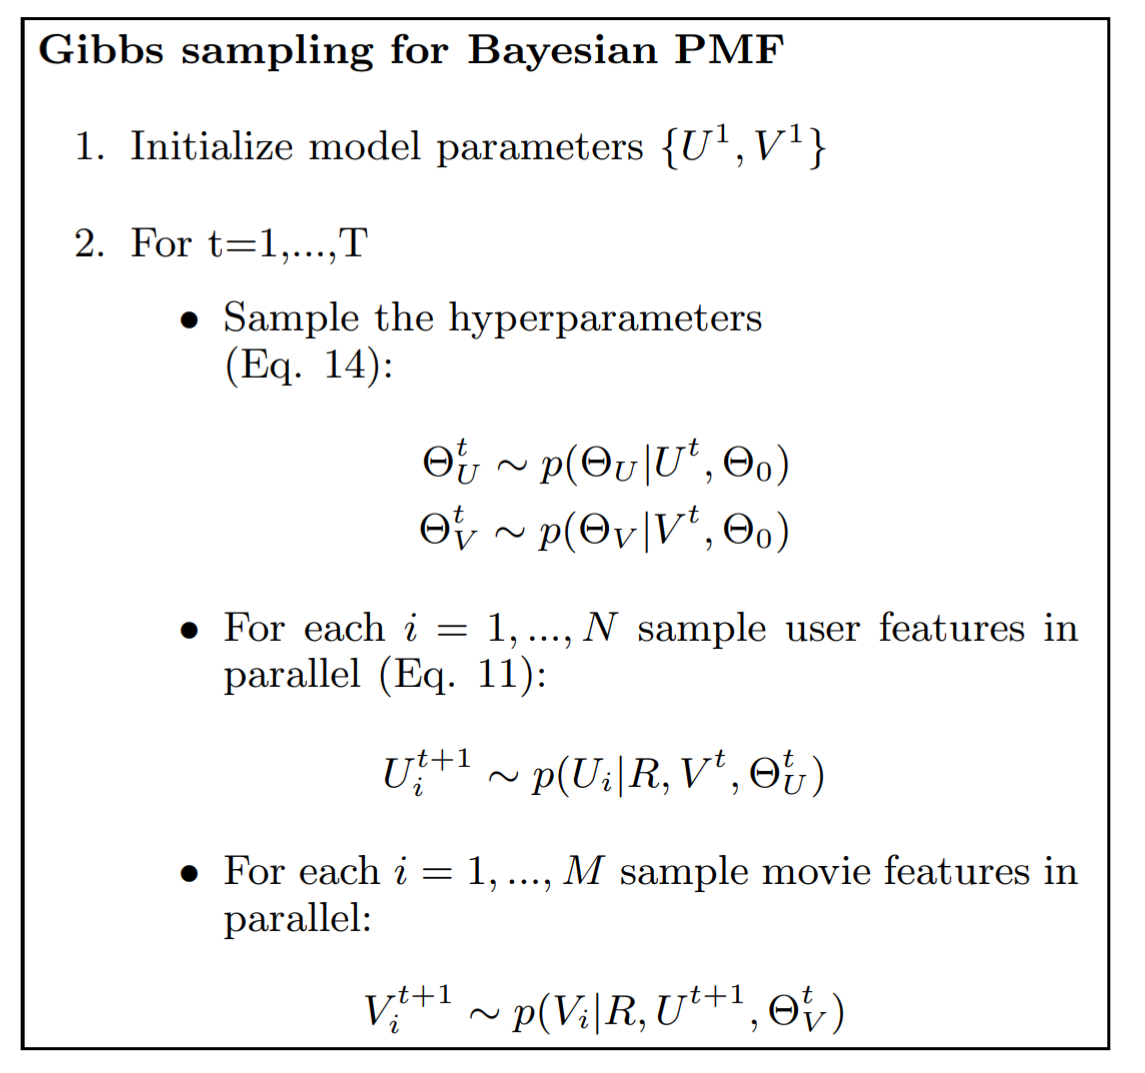
\includegraphics[scale=0.35]{gibbs.png}
\caption{Gibbs sampling algorithm as shown in \cite{BPMF}}
\label{gibbs}
\end{figure} 

\item[\emph{NPCA}] \ \\
NPCA is an extension of Probabilistic PCA which deals with infinitely many latent factors. We implemented the model following \cite{npca}. In this situation, working directly with the vector of latent factors $\textbf{u}$ and $\textbf{v}$ is intractable and the vector $\textbf{x}_i = \left[u_i^Tv_1, \dots , u_i^Tv_j, \dots , u_i^Tv_N \right] $ is used instead. The model then describes a latent process $X$ and an observational one $Y$ described by the following distribution:
$$
\int p(Y,X \vert K, \lambda)dX = \prod_{i=1}^M \mathcal{N}(y_{\mathbb{O}_i};0, K_{\mathbb{O}_i} + \lambda I)
$$

\noindent where Y is the user-item matrix, K and lambda some hyperparameters, and $\mathbb{O}_{i}$ the indices of the observed items for a given user $i$. This equation is maximized using an EM algorithm. The authors formalize a fast EM algorithm that avoids computing an NxN inverse matrix called Fast NPCA which is depicted in \emph{Figure \ref{emnpca}}.

\begin{figure}[t!]
\centering
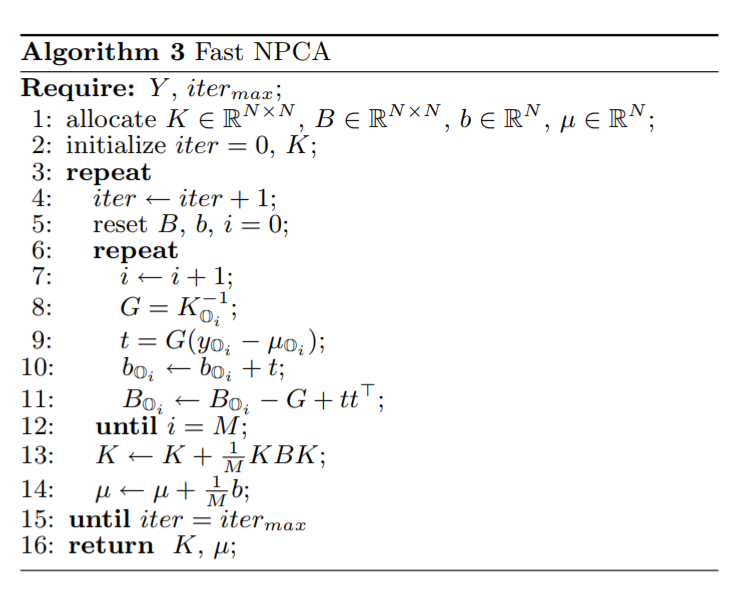
\includegraphics[scale=0.6]{emnpca.png}
\caption{Fast NPCA EM algorithm as shown in \cite{npca}}
\label{emnpca}
\end{figure} 

\item[Autoencoder] \ \\
An autoencoder provides a method to lean a non-linear mapping from $\mathbb{R}^{m}$ to $\mathbb{R}^{m}$. As shown in \cite{autorec}, this neural network can be adapted to the problem of collaborative filtering determined by a user-item rating matrx $M \times N$, by using each partially observed item vector $I_{i} \in {R}^{m} , i \in \{1,...n\}$ (\emph{Figure \ref{autoenc}}).

\begin{figure}[t!]
\centering
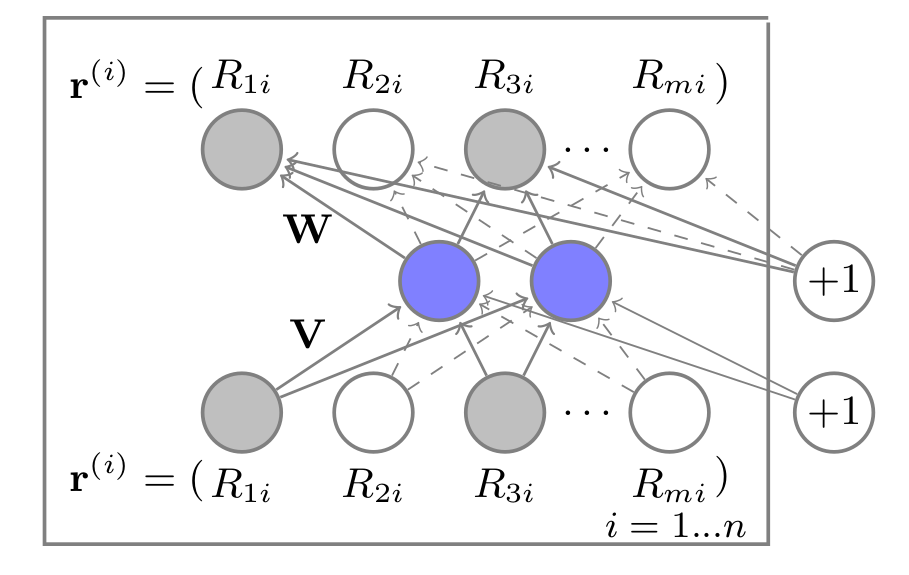
\includegraphics[scale=0.25]{autoenc.png}
\caption{Autoencoder for collaborative filtering \cite{autorec}}
\label{autoenc}
\end{figure} 
A random number set of observed ratings of $I_{i}$ will then be set to 0, corresponding to a non-observed rating. The objective function formalizes then a linear combination of the L2-error on the predicted output for these hidden values, and the L2-error on the output of the initially observed ratings.
As suggested in \cite{DBLP:journals/corr/StrubMG16}, the loss function will then be: 
$$
\begin{aligned}
L_{2,\alpha,\beta}(x,\widetilde{x}) = \alpha(\sum\limits_{j \in \mathcal{C}(\widetilde{x})} [nn(\widetilde{x})_{j}]^{2})+ \\ \beta(\sum\limits_{j \notin \mathcal{C}(\widetilde{x})} [nn(\widetilde{x})_{j}]^{2})
\end{aligned}
$$
where $\widetilde{x}$ is the corrupted version of $x$ and $nn(\widetilde{x}_j)$ is the $j^{th}$ of the network fed with $x$. 
\newline
Additionaly to adding L2-regularization terms for the network weights, we corrupt the input further as suggested in \cite{Vincent:2010:SDA:1756006.1953039}. Before hidding some part of the input, we first add random gaussian noise and what the authors call "salt and pepper" noise, which consists of randomly putting some elements to the minimum rating and some to the maximum rating.
\newline 
Finally, we also tested the possibility to add more layers to the autoencoder to learn more complex features as proposed in \cite{Kuchaiev2017TrainingDA}. 

\end{description}

\subsection{Ensemble}
The performance of an invidual model can depend on multiple factors like the size of the rating matrix, its sparsity and other non-obvious parameters \cite{comparative}. 
To be able to combine the strength of each individual model, we determined the optimal linear combination of the predictions made by these models on a validation set. 
\[
\begin{bmatrix}
    pred_{1,1}  & \hdots & pred_{1,m}\\
    pred_{2,1}  & \hdots & pred_{2,m}\\
    \hdotsfor{3} \\
    pred_{d,1}  & \hdots & pred_{d,m}
\end{bmatrix}
\begin{bmatrix}
    w_{1}\\
    \hdots \\
    w_{m}\\
\end{bmatrix}
=
\begin{bmatrix}
    val_{1}\\
    val_{2}\\
    \hdotsfor{1} \\
    val_{d}
\end{bmatrix}
\]
where the d predictions of the m models are linearly combined. We also added a L2-regularization term to avoid overfitting on the validation set. 
\newline
We also combined the features using a Multi Layer Perceptron, using the rows of the above left matrix as training input. Due to the complexity of this model, the variance had to be generously regularized. 
\newline
The results have been showing that it was essential to keep a small part of the training data exclusively for model combining so that the trained models can be combined over true validation data.  

\section{Evaluation}
\label{res}

\subsection{Set-up}

Our dataset comprises 10000 users and 1000 movies. The results are computed by submitting the predictions to the Kaggle platform, which, as mentioned in \emph{Problem Description}, evaluates the prediction error via RMSE.

\subsection{Results}

We present the results of single models in \emph{Table \ref{tabres}} and of the two types of ensemble methods in \emph{Table \ref{ensres}}. We discuss them in the following section.

\begin{table}[h!]
	\centering
	\begin{tabular}{l|l}
		\textit{\textbf{Model}} & \textit{\textbf{RMSE}} \\
		\hline
		SVD                     &       1.00468                 \\
		SVD + SGD               &                        \\
		RSVD       	            &        0.98787                \\
		Ridge SVD               &        1.0264                \\
		Item-Based              &        1.05                \\
		k-means                 &        1.06                \\
		BPMF                    &        0.99695               \\
		NPCA                    &        1.0264          \\
		AutoEncoder             &        0.996               
	\end{tabular}
\caption{Results of our models' evaluation}
\label{tabres}
\end{table}

\begin{table}[h!]
	\centering
	\begin{tabular}{l|l}
		\textit{\textbf{Ensemble}} & \textit{\textbf{RMSE}} \\
		\hline
		Ridge                     &      0.97858                 \\
		MLP      	            &         0.97518                                   
	\end{tabular}
\caption{Results of our ensemble methods' evaluation}
\label{ensres}
\end{table}

\section{Discussion}
\label{disc}

\emph{Table \ref{tabres}} shows the results obtained by evaluation of each single model submitting the predictions to the Kaggle system. As can be seen, the best result in terms of RMSE on the given dataset is obtained applying RSVD with a score of 0.98787, meaning an improvement of 1.67\% with respect to the baseline (TODO CHECK BASELINES VALUES), while the worst is obtained by k-means with a score of 1.06, which corresponds to a deterioration of 5.51\%. However, as mentioned in both \emph{Section \ref{int}} and \emph{Section \ref{mam}}, individual models can have several limitations and thus, to overcome this factor, we implemented and evaluated two types of ensemble models. The results of such models are represented in \emph{Table \ref{ensres}}. As can be seen, ensemble with Ridge regression scored a RMSE value of 0.97858, corresponding to an improvement of 2.6\% with respect to the baseline, of 7.68\% to the worst model (\emph{i.e.}, k-means) and of 0.94\% to the best individual model (\emph{i.e.}, RSVD). Using the MLP regressor, we could lower even further the results scoring a value of 0.97518, meaning a further improvement of 0.35\% with respect to the Ridge ensemble. Comparing the best result to individual models, we have an improvement of 2.94\%, 8\% and 1.28\% with respect to the baseline, k-means and the RSVD models respectively. We further summarize these findings in \emph{Table \ref{sumtab}} and \emph{Table \ref{enssum}}.

\begin{table}[h!] 
	\centering
	\begin{tabular}{l|c|c}
		\textit{\textbf{Individual Model}} & \textit{\textbf{RRE Improvement}} & \textit{\textbf{MLPE Improvement}} \\
		\hline
		SVD                     &       2.6\%     &     2.94\%         \\
		SVD + SGD               &                 &      				 \\
		RSVD       	            &        0.94\%  &     1.28\%         		\\
		Ridge SVD               &        4.66\%   &    4.99\%         		\\
		Item-Based              &        6.8\%     &   7.13\%        		\\
		k-means                 &        7.68\%     &  8.00\%         		\\
		BPMF                    &        1.84\%  &     2.18\%        \\
		NPCA                    &        4.66\%   &    4.99\%   				\\
		AutoEncoder             &        1.75\%    &   2.09\%        
	\end{tabular}
    \caption{Summary of the improvements achieved using ensemble models}
    \label{sumtab}
\end{table}

\begin{table}[h!]
	\centering
	\begin{tabular}{l|c}
		\textit{\textbf{Ensemble}} & \textit{\textbf{MLPE Improvement}} \\
		\hline
		Ridge                     &      0.35\%                 \\                              
	\end{tabular}
\caption{Improvement of MLP over RR ensemble.}
\label{enssum}
\end{table}

\section{Conclusions}
\label{conc}

In this work we implemented and evaluated different Collaborative Filtering techniques to build reliable and efficient Recommender Systems. We first implemented 7 different individual models based on different papers and submitted their predictions to the Kaggle system to be able to compare their performances in terms of the Root Mean Squared Error, and analyse their strengths and limitations. To further improve the predictions, we implemented and tested two different types of ensemble models, the first using Ridge Regression and the second using a Multi-Layer Perceptron. Analysing both methods' predictions, we concluded that the latter was the best model in our situation. By using this approach, we were able to further enhance our results achieving a final score of 0.97518, corresponding to a final improvement of 1.28\% over our best individual model (RSVD), of 8.00\% with respect to the worst model (k-means), and of 0.35\% with respect to the first ensemble model.


\bibliographystyle{IEEEtran}
\bibliography{biblio}
\end{document}
